%!TEX TS-program = xelatex
\documentclass[12pt, a4paper, oneside]{article}

% Можно вставить разную преамбулу
% пакеты для математики
\usepackage{amsmath,amsfonts,amssymb,amsthm,mathtools}  
\mathtoolsset{showonlyrefs=true}  % Показывать номера только у тех формул, на которые есть \eqref{} в тексте.

\usepackage[british,russian]{babel} % выбор языка для документа
\usepackage[utf8]{inputenc}          % utf8 кодировка

% Основные шрифты 
\usepackage{fontspec}         
\setmainfont{Linux Libertine O}  % задаёт основной шрифт документа

% Математические шрифты 
\usepackage{unicode-math}     
\setmathfont[math-style=upright]{euler.otf} 

\setmathfont[range={\mathbb, \mathop, \heartsuit, \angle, \smile, \varheartsuit}]{Asana-Math.otf}

%%%%%%%%%% Работа с картинками и таблицами %%%%%%%%%%
\usepackage{graphicx} % Для вставки рисунков                
\usepackage{graphics}
\graphicspath{{images/}{pictures/}}   % папки с картинками

\usepackage[figurename=Картинка]{caption}

\usepackage{wrapfig}    % обтекание рисунков и таблиц текстом

\usepackage{booktabs}   % таблицы как в годных книгах
\usepackage{tabularx}   % новые типы колонок
\usepackage{tabulary}   % и ещё новые типы колонок
\usepackage{float}      % возможность позиционировать объекты в нужном месте
\renewcommand{\arraystretch}{1.2}  % больше расстояние между строками


%%%%%%%%%% Графики и рисование %%%%%%%%%%
\usepackage{tikz, pgfplots}  % языки для графики
%\pgfplotsset{compat=1.16}

\usepackage{todonotes} % для вставки в документ заметок о том, что осталось сделать
% \todo{Здесь надо коэффициенты исправить}
% \missingfigure{Здесь будет Последний день Помпеи}
% \listoftodos --- печатает все поставленные \todo'шки

\usepackage{multicol}

%%%%%%%%%% Внешний вид страницы %%%%%%%%%%

\usepackage[paper=a4paper, top=20mm, bottom=15mm,left=20mm,right=15mm]{geometry}
\usepackage{indentfirst}    % установка отступа в первом абзаце главы

\usepackage{setspace}
\setstretch{1.15}  % межстрочный интервал
\setlength{\parskip}{4mm}   % Расстояние между абзацами
% Разные длины в LaTeX: https://en.wikibooks.org/wiki/LaTeX/Lengths

% свешиваем пунктуацию
% теперь знаки пунктуации могут вылезать за правую границу текста, при этом текст выглядит ровнее
\usepackage{microtype}

% \flushbottom                            % Эта команда заставляет LaTeX чуть растягивать строки, чтобы получить идеально прямоугольную страницу
\righthyphenmin=2                       % Разрешение переноса двух и более символов
\widowpenalty=300                     % Небольшое наказание за вдовствующую строку (одна строка абзаца на этой странице, остальное --- на следующей)
\clubpenalty=3000                     % Приличное наказание за сиротствующую строку (омерзительно висящая одинокая строка в начале страницы)
\tolerance=10000     % Ещё какое-то наказание.

% мои цвета https://www.artlebedev.ru/colors/
\definecolor{titleblue}{rgb}{0.2,0.4,0.6} 
\definecolor{blue}{rgb}{0.2,0.4,0.6} 
%\definecolor{red}{rgb}{1,0,0.2} 
\definecolor{green}{rgb}{0, 0.6, 0}
\definecolor{purp}{rgb}{0.4,0,0.8} 

\definecolor{red}{RGB}{213,94,0}
\definecolor{yellow}{RGB}{240,228,66}


% цвета из geogebra 
\definecolor{litebrown}{rgb}{0.6,0.2,0}
\definecolor{darkbrown}{rgb}{0.75,0.75,0.75}

% Гиперссылки
\usepackage{xcolor}   % разные цвета

\usepackage{hyperref}
\hypersetup{
	unicode=true,           % позволяет использовать юникодные символы
	colorlinks=true,       	% true - цветные ссылки
	urlcolor=blue,          % цвет ссылки на url
	linkcolor=black,          % внутренние ссылки
	citecolor=green,        % на библиографию
	breaklinks              % если ссылка не умещается в одну строку, разбивать её на две части?
}

% меняю оформление секций 
\usepackage{titlesec}
\usepackage{sectsty}

% меняю цвет на синий
\sectionfont{\color{titleblue}}
\subsectionfont{\color{titleblue}}

% кружочки у цифр в секциях
\renewcommand{\thesection}{\arabic{section}}

% https://ru.overleaf.com/learn/latex/Sections_and_chapters

% выбрасываю нумерацию страниц и колонтитулы 
%\pagestyle{empty}

% синие круглые бульпоинты в списках itemize 
\usepackage{enumitem}

\definecolor{itemizeblue}{rgb}{0, 0.45, 0.70}

\newcommand*{\MyPoint}{\tikz \draw [baseline, fill=itemizeblue, draw=blue] circle (2.5pt);}
\renewcommand{\labelitemi}{\MyPoint}

\AddEnumerateCounter{\asbuk}{\@asbuk}{\cyrm}
\renewcommand{\theenumi}{\asbuk{enumi}}

% расстояние в списках
\setlist[itemize]{parsep=0.4em,itemsep=0em,topsep=0ex}
\setlist[enumerate]{parsep=0.4em,itemsep=0em,topsep=0ex}

% эпиграфы
\usepackage{epigraph}
\setlength\epigraphwidth{.6\textwidth}
\setlength\epigraphrule{0pt}

%%%%%%%%%% Свои команды %%%%%%%%%%

% Математические операторы первой необходимости:
\DeclareMathOperator{\sgn}{sign}
\DeclareMathOperator*{\argmin}{arg\,min}
\DeclareMathOperator*{\argmax}{arg\,max}
\DeclareMathOperator{\Cov}{Cov}
\DeclareMathOperator{\Var}{Var}
\DeclareMathOperator{\Corr}{Corr}

\DeclareMathOperator{\Pois}{Pois}
\DeclareMathOperator{\Geom}{Geom}
\DeclareMathOperator{\Exp}{Exp}

%\DeclareMathOperator{\E}{\mathbb{E}}
\DeclareMathOperator{\Med}{Med}
\DeclareMathOperator{\Mod}{Mod}
\DeclareMathOperator*{\plim}{plim}

% команды пореже
\newcommand{\const}{\mathrm{const}}  % const прямым начертанием
\newcommand{\iid}{\sim i\,i\,d\,\,}  % ну вы поняли...
\newcommand{\fr}[2]{\ensuremath{^{#1}/_{#2}}}   % особая дробь
\newcommand{\ind}[1]{\mathbbm{1}_{\{#1\}}} % Индикатор события
\newcommand{\dx}[1]{\,\mathrm{d}#1} % для интеграла: маленький отступ и прямая d

% одеваем шапки на частые штуки
\def \hb{\hat{\beta}}
\def \hs{\hat{s}}
\def \hy{\hat{y}}
\def \hY{\hat{Y}}
\def \he{\hat{\varepsilon}}
\def \hVar{\widehat{\Var}}
\def \hCorr{\widehat{\Corr}}
\def \hCov{\widehat{\Cov}}

% Греческие буквы
\def \a{\alpha}
\def \b{\beta}
\def \t{\tau}
\def \dt{\delta}
\def \e{\varepsilon}
\def \ga{\gamma}
\def \kp{\varkappa}
\def \la{\lambda}
\def \sg{\sigma}
\def \tt{\theta}
\def \Dt{\Delta}
\def \La{\Lambda}
\def \Sg{\Sigma}
\def \Tt{\Theta}
\def \Om{\Omega}
\def \om{\omega}

% Готика
\def \mA{\mathcal{A}}
\def \mB{\mathcal{B}}
\def \mC{\mathcal{C}}
\def \mE{\mathcal{E}}
\def \mF{\mathcal{F}}
\def \mH{\mathcal{H}}
\def \mL{\mathcal{L}}
\def \mN{\mathcal{N}}
\def \mU{\mathcal{U}}
\def \mV{\mathcal{V}}
\def \mW{\mathcal{W}}

% Жирные буквы
\def \mbb{\mathbb}
\def \RR{\mbb R}
\def \NN{\mbb N}
\def \ZZ{\mbb Z}
\def \PP{\mbb{P}}
\def \E{\mbb{E}}
\def \QQ{\mbb Q}

\def\F{\ensuremath{\mathcal{F}}} % аналогично!

%%%%%%%%%% Теоремы %%%%%%%%%%
\theoremstyle{plain} % Это стиль по умолчанию.  Есть другие стили.
\newtheorem{theorem}{Теорема}[section]
\newtheorem{proposition}{Утверждение}[section]
\newtheorem{result}{Следствие}[section]

% убирает курсив и что-то еще наверное делает ;)
\theoremstyle{definition}         
\newtheorem*{definition}{Определение}  % нумерация не идёт вообще


%%%%%%%%%% Задачки и решения %%%%%%%%%%
\usepackage{etoolbox}    % логические операторы для своих макросов
\usepackage{environ}
\newtoggle{lecture}

\newcounter{probNum}[section]  % счётчик для упражнений 
\NewEnviron{problem}[1]{%
    \refstepcounter{probNum}% увеличели номер на 1 
    {\noindent \textbf{\large \color{titleblue} Упражнение~\theprobNum~#1}  \\ \\ \BODY}
    {}%
  }

% Окружение, чтобы можно было убирать решения из pdf
\NewEnviron{sol}{%
  \iftoggle{lecture}
    {\noindent \textbf{\large Решение:} \\ \\ \BODY}
    {}%
  }
 
% выделение по тексту важных вещей
\newcommand{\indef}[1]{\textbf{ \color{green} #1}} 

% разные дополнения для картинок
\usetikzlibrary{arrows.meta}
\usepackage{varwidth}

\usepackage[normalem]{ulem}  % для зачекивания текста

% Если переключить в false, все solution исчезнут из pdf
\toggletrue{lecture}
%\togglefalse{lecture}



\title{
\begin{center} 
\includegraphics[width=0.99\textwidth]{logo.png}
\end{center}

Посиделка 8: мощь средних}
\date{ } %\today}

% Если делаешь конспект, вписывай своё имя прямо сюда!
\author{Ульянкин Ппилиф \thanks{\url{https://github.com/FUlyankin/matstat_lec}}}

\begin{document} % Конец преамбулы, начало файла

\maketitle

\epigraph{\hfill Бесконечность --- не предел!}{\textit{Баз Лайтер (История игрушек, 1995)}}

Когда мы обсуждали в первой посиделке схему матстата, мы сказали, что существует несколько разных подходов к построению моделей. У каждого из них есть своя изюминка. В этой посиделке мы попробуем построить матстат на базе среднего. 

\begin{center}
    \begin{tikzpicture}[scale = 1.5, line cap=round,line join=round,x=1.0cm,y=1.0cm]
    
        \path (-1,0) node(x) {\Huge $\hat \theta$} (3,0) node(y) {\Huge $f_{\hat \theta} (t)$};
        
        \node at (8, 0) {\footnotesize
            \begin{varwidth}{\linewidth}\begin{itemize}
                \item прогнозы
                \item насколько точны прогнозы
                \item ответы на вопросы (гипотезы)
            \end{itemize}\end{varwidth}
        };
        
        \draw[->, line width=1.1pt] (-0.5,0) -- (2,0);
        \draw[->, line width=1.1pt] (4,0) -- (6,0);
    
        \node at (-0.2, -1.45) { \footnotesize
            \begin{varwidth}{\linewidth} \textbf{Cоюзники:}
            \begin{itemize}
                \item метод моментов 
                \item обобщённый метод моментов
            \end{itemize}\end{varwidth}
        };
        
        \node at (4.5, -1.45) { \footnotesize
            \begin{varwidth}{\linewidth} \textbf{Cоюзники:}
            \begin{itemize}
                \item центральная предельная теорема (ЦПТ)
                \item Дельта-метод
            \end{itemize}\end{varwidth}
        };
    \end{tikzpicture}
\end{center} 

Искать точечные оценки мы будем с помощью метода моментов, который основан на законе больших чисел (ЗБЧ). Искать распределение оценки нам поможет центральная предельная теорема (ЦПТ). В следующей посиделке мы обобщим ЦПТ до дельта-метода, а метод моментов до обобщённого метода моментов. 

\section{Метод моментов и ЗБЧ}

Пусть случайные величины $X_{1}, \ldots, X_{n}$ независимы и одинаково распределены. Закон больших чисел говорит нам, что среднее выборочное $\bar{X}$ является хорошей оценкой для математического ожидания $ \E(X_{i}) $.

\begin{theorem}{\textbf{Закон Больших Чисел (Пафнутий Львович Чебышёв)}}

Пусть $X_1, \ldots, X_n$ попарно независимые и одинаково распределённые случайные величины с конечным вторым моментом, $0 < E(X_i^2) < \infty$, тогда:

$$
\bar{X}_{n} = \frac{X_1 + \ldots + X_n}{n} \stackrel{p}{\longrightarrow} E(X_1)
$$
\end{theorem}

На практике это означает, что при больших $n$ эти величины примерно равны:

\[
\bar{X}_{n} \approx \E(X_{i}).
\]

На этой нехитрой идее и построен метод моментов. Как конкретно используется идея, понятно из следующих нескольких примеров.

\begin{problem}{(киндеры)}
    Максим любит киндеры и собирает коллекцию пляжных бегемотиков. Для этого он покупает шоколадки. Пусть $p$ --- вероятность того, что в киндере лежит пляжный бегемотик. Максим покупает яйца и записывает номер попытки, с которой у него появилась правильная игрушка.
    
    До первого бегемотика Максим купил $X_1$ яиц. После счётчик обнулился. До второго бегемотика Макс купил $X_2$ яиц и так далее. Всего Макс собрал $n$ бегемотиков. Постройте оценку неизвестного параметра $p$ с помощью метода моментов.
\end{problem}

\begin{sol}
\indef{Эксперимент} состоит в том, что Максим ест шоколад и собирает \indef{выборку} из своих попыток раздобыть нужную игрушку. \indef{Вопрос Макса} заключается в том, насколько часто встречаются бегемотики. \indef{Модель Макса,} в которую он верит заключается в том, что величины $X_{i}$ имеют геометрическое распределение, поэтому $\E(X_{i})=\frac{1}{p}$. Принцип метода моментов гласит:
	\[ \bar{X}_{n}\approx \frac{1}{p}.\]
	Выражаем неизвестный параметр $ p $:
	\[ p\approx \frac{1}{\bar{X}_{n}}. \]
	Это и есть нужная нам оценка:
	\[ \hat{p}_{MM} = \frac{1}{\bar{X}_{n}}. \]
\end{sol}


\begin{problem}{(Шарик и фарш)}
Продавщица Глафира отдаёт псу Шарику в конце каждого дня нерасфасованные остатки мясного фарша. Фарш фасуется упаковками по $a$ грамм, поэтому нерасфасованный остаток в $i$-ый день, $X_i$, случаен и равномерно распределен на отрезке $[0;a]$. Пёс Шарик хорошо помнит все $X_1$, \ldots, $X_n$. Помогите псу Шарику найти оценку $a$ методом моментов.
\end{problem}

\begin{sol}
\indef{Эксперимент} состоит в том, что Шарик каждый день ест фарш и собирает \indef{выборку.} \indef{Вопрос Шарика} заключается в том, сколько максимально фарша он может получить. \indef{Модель Шарика,} в которую он верит --- выборка приходит из равномерно распределения. В рамках этой веры мы пробуем решить задачу.

В данном случае $ \E(X_{i})=\frac{a}{2} $ и, следовательно
\[ \bar{X}_{n}\approx \frac{a}{2}. \]
Выражаем $a$
\[ a \approx 2 \cdot \bar{X}_{n}, \]
это и есть нужная нам оценка:
\[ \hat{a}^{MM}= 2 \cdot \bar{X}_{n}. \]
\end{sol}

\begin{definition} 
Пусть $X_1, \ldots, X_n$ одинаково распределены и независимы, а $\E(X_{i})$ зависит от неизвестного параметра $\theta$, скажем $\E(X_{i}) = f(\theta)$. Тогда \indef{оценкой метода моментов} называется случайная величина:
\[ \hat{\theta}_{MM} = f^{-1}(\bar{X}_{n}) \]
\end{definition} 

Конечно, иногда бывают ситуации, когда математическое ожидание $\E(X_{i})$ не зависит от $\theta$. Например, если $X_{i}$ равномерны на $[-\theta; \theta]$, то математическое ожидание $\E(X_{i}) = 0$. Что делать в такой ситуации? 

Неспроста же наш метод называется методом моментов\ldots{}  Напомним, что $k$-ым моментом случайной величины $X_{i}$ называется математическое ожидание $\E(X_{i}^{k})$. 

Если условия $\bar{X}_{n}\approx \E(X_{i}),$ связанного с первым моментом не хватило, то на помощь придет второй момент случайной величины. В силу того же закона больших чисел:

\[\overline{X^2}_n = \frac{X_{1}^{2} + \ldots + X_{n}^{2}}{n} \approx \E(X_{i}^{2})\]

\begin{problem}{(равномерное)}
Величины $ X_{i} $ независимы и равномерны на $ [-\theta;\theta] $. Постройте оценку неизвестного параметра $\theta$ с помощью метода моментов.
\end{problem}

\begin{sol}
Убеждаемся, что $\E(X_{i})=0$:

\[  \E(X_{i}) = \int _{-\theta}^{\theta} x \cdot \frac{1}{2\theta} \dx{x} = \left. \frac{x^2}{4 \theta} \right|_{-\theta}^{\theta} = \left( \frac{\theta^2 - (-\theta)^2 }{4 \theta}  \right) =  \frac{\theta^{2} - \theta^{2}}{4 \theta} = 0  \]

Находим $ \E(X_{i}^{2}) $:

\[  \E(X_{i}^{2}) = \int _{-\theta}^{\theta} x^{2} \cdot \frac{1}{2\theta}  \dx{x} = \left. \frac{x^3}{6 \theta} \right|_{-\theta}^{\theta} = \left( \frac{\theta^3 - (-\theta)^3 }{6\theta}  \right) = \frac{2 \theta^{3}}{6\theta}  = \frac{\theta^{2}}{3}  \]

Согласно принципу метода моментов

\[ \frac{\sum X_{i}^{2}}{n} \approx \frac{\theta^{2}}{3}.\]

Выражаем $ \theta $

\[ \theta\approx \sqrt{3\frac{\sum X_{i}^{2}}{n} }.\]

Это и есть нужная нам оценка

\[ \hat{\theta}_{MM}= \sqrt{3\frac{\sum X_{i}^{2}}{n} } = \sqrt{3 \overline{X^2 } }.\]
\end{sol}

Если не хватит и второго момента, тогда воспользуемся третьим и т.д. Для произвольного $k$ мы имеем

\[ \frac{X_{1}^{k} + \ldots + X_{n}^{k}}{n} \approx \E(X_{i}^{k})\]

В большинстве случаев хватает именного первого момента. Последующие моменты нужны чаще всего при оценке нескольких параметров.

\begin{problem}{(Нормальное)}
Исследователь Мстислав собрал выборку $X_1, \ldots, X_n$ из нормального распределения $\mN(\mu, \sigma^2)$ и теперь хочет методом моментов оценить неизвестные параметры. Нужно ему помочь в этом нелёгком деле.
\end{problem}

\begin{sol}
У нас два параметра. Будем использовать два уравнения

\[
\begin{cases} 
\E(X^2) \approx \overline{X^2}_n   \\
\E(X^2) \approx  \bar{X}_n 
\end{cases} \Leftrightarrow \begin{cases} 
\sigma^2 + \mu \approx \overline{X^2}_n   \\
 \mu \approx \bar{X}_n
\end{cases}  \Leftrightarrow \begin{cases} 
 \hat{\sigma}^2 = \overline{X^2}_n - \hat{\mu} = \overline{X^2}_n - \bar{X}_n \\
\hat{\mu} = \bar{X}_n.
\end{cases}
\]

Обратите внимание, что колпачок над параметрами появляется в тот момент, когда мы строго приравниваем математическое ожидание к среднему. Начиная с этого момента мы имеем дело с оценками. Для реального распределение значение математических ожиданий может отличаться от средних, посчитанных по конкретным выборкам. 
\end{sol} 


% \begin{problem}{(Задача о Танках)}


% \end{problem}
% \begin{sol}

% \end{sol} 

\section{ЦПТ и асимптотические доверительные интервалы}

Точечная оценка --- это хорошо. К сожалению, чаще всего нам этого мало. Всегда хочется понимать, насколько оценка получилась точной. Нам в этом помогают \indef{доверительные интервалы,} то есть промежутки, которые накрывают истинное значение параметра с высокой вероятностью. Построить доверительные интервалы нам помогает союзник, ЦПТ.

\begin{theorem}{\textbf{Центральная Предельная Теорема (Прокопий Петрович Ляпунов)}}

Пусть $X_1, \ldots, X_n$ попарно независимые и одинаково распределённые случайные величины с конечным вторым моментом, $0 < E(X_i^2) < \infty$, тогда при $n \to \infty$ имеет место сходимость по распределению: 
\[
\bar{X}_n \stackrel{d}{\longrightarrow} \mN \left(\E(X_i), \frac{\Var(X_i)}{n} \right)
\]
Этот же факт можно переписать немного иначе
\[
\sqrt{n} \cdot [\bar{x} - \E(X_i)]  \stackrel{d}{\longrightarrow} \mN \left(0, \Var(X_i)\right)
\]
или даже 
\[
\sqrt{n} \cdot \frac{\bar{x} - \E(X_i)}{\sqrt{\Var(X_i)}}  \stackrel{d}{\longrightarrow} \mN \left(0, 1\right).
\]
\end{theorem}
Если говорить простым языком, то при определённых условиях сумма достаточно большого числа случайных величин имеет распределение близкое к нормальному. \indef{Главное, чтобы случайные величины были похожи и не было такого, что одна резко выделяется на фоне~остальных.}


\begin{problem}{(Шарик и фарш)}
Величины $X_1$, \ldots, $X_n \iid U[0;a]$. Найдите для $a$ оценку методом моментов и постройте для неё доверительный интервал. У Шарика есть гипотеза, что вес упаковки не может превышать $100$ грамм. Формализуйте эту гипотезу и опишите процедуру её проверки. 
\end{problem}

\begin{sol}
Мы нашли оценку метода моментов, оказалось что 
\[ \hat{a} = 2 \cdot \bar{X}_{n}. \]

В данном случае мы работаем с равномерным распределением, а значит $\Var(X_i) = \frac{a^2}{12}.$ Получается, что $\Var(\bar X_n) = \frac{a^2}{12 \cdot n}.$ Воспользовавшись ЦПТ мы можем выписать асимптотическое распределение среднего 

\[\bar{X}_n \overset{\text{\textit{asy}}}{\sim} \mN \left(\frac{a}{2}, \frac{a^2}{12 \cdot n} \right).\] 

По свойствам нормального распределения, получаем распределение для оценки неизвестного параметра

\[\hat{a}= 2 \bar{X}_{n} \overset{\text{\textit{asy}}}{\sim} \mN \left(a, \frac{a^2}{3 \cdot n} \right).\] 

Математическим ожиданием нашей оценки является сам параметр. Это говорит о том, что оценка получилась несмещённой. Нам хочется понять, насколько оценка точная. Для этого нужно знать дисперсию. В ней фигурирует неизвестное значение $a$. Его смело можно заменить на оценку $\hat{a}$. Асимптотика от этого никак не испортится. Чуть позже мы это докажем. 
\[
\hat{a}= 2 \bar{X}_{n} \overset{\text{\textit{asy}}}{\sim} \mN \left(a, \frac{4 \bar{X}^2}{3 \cdot n} \right).
\] 

Давайте запишем для случайной величины $\hat a$ интервал, в котором она лежит с вероятностью $0.95.$ По правилу двух сигм получаем
\[
\PP \left(a - 2 \cdot \sqrt{\frac{4 \bar{X}^2}{3 \cdot n}}  \le \hat a \le a + 2 \cdot \sqrt{\frac{4 \bar{X}^2}{3 \cdot n}} \right) = 0.95.
\]

Такой интервал для случайной величины $\hat a$ называется \indef{предиктивным интервалом.} Его границы фиксированы, а в центре находится случайная величина. Давайте разрешим неравенство относительно $a$. Вычтем из каждой части $a$ и домножим на $-1.$ Тогда мы получим, что
\[
\PP \left(\hat a - 2 \cdot \sqrt{\frac{4 \bar{X}^2}{3 \cdot n}}  \le a \le \hat a + 2 \cdot \sqrt{\frac{4 \bar{X}^2}{3 \cdot n}} \right) = 0.95.
\]

Такой интервал называется \indef{доверительным интервалом.} Его границы --- случайные величины, а в середине стоит неизвестная константа, которую доверительный интервал накрывает с вероятностью $0.95$. Если мы соберём много-много выборок и построим по каждой доверительный интервал, он в $95\%$ ситуаций накроет $a$.

Если доверительный интервал оказывается очень широким, значит наша оценка неточная. Обратите внимание, что мы используем для строительства доверительного интервала ЦПТ. Её предпосылки должны выполнятся для выборки. Если это не так, интервал будет некорректным.

Давайте построим доверительный интервал, который будет покрывать неизвестный параметр с вероятностью $1 - \alpha.$ Эта вероятность называется \indef{уровнем доверия.} Величина $\alpha$ называется \indef{уровнем значимости.} Это тот же самый уровень значимости, о котором мы говорили в первых посиделках. 

Давайте вычтем из $\hat a$ математическое ожидание и поделим разность на стандартное отклонение. Получившаяся случайная величина будет иметь стандартное нормальное распределение
\[
Z = \frac{ 2 \bar{X}_{n} - a}{\sqrt{\frac{4 \bar{X}^2}{3 \cdot n}} } \overset{\text{\textit{asy}}}{\sim} \mN \left(0, 1 \right).
\] 

Попробуем понять насколько точной получилась наша оценка. Зажмём случайную величину $Z$ между её квантилями так, чтобы 

\[
\PP \left( z_{1 - \frac{\alpha}{2}} \le Z \le z_{1 - \frac{\alpha}{2}} \right) = 1 - \alpha.
\]

\begin{center} 
    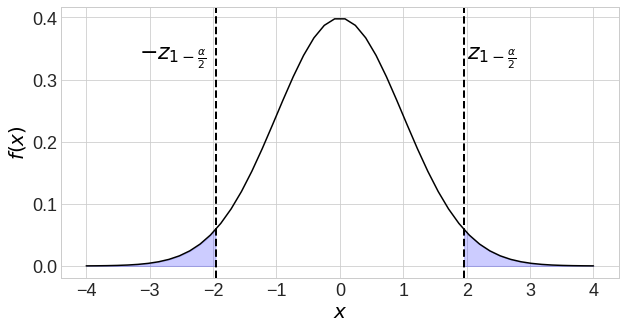
\includegraphics[width=0.7\linewidth]{conf_int_asy.png}
\end{center} 

Выбирая $\alpha$ мы выбираем для случайной величины $Z$ с двух сторон засечки. Между ними с вероятностью $1 - \alpha$ лежит рассматриваемая случайная величина. Если разрешить неравенство относительно $a,$ мы получим доверительный интервал 

$$
\PP\left(2 \bar{X}_{n}  - z_{1 - \frac{\alpha}{2}} \cdot \sqrt{\frac{4 \bar{X}^2}{3 \cdot n}}  \le a \le 2 \bar{X}_{n}  + z_{1 - \frac{\alpha}{2}} \cdot \sqrt{\frac{4 \bar{X}^2}{3 \cdot n}} \right) = 1 - \alpha.
$$

По аналогии мы можем построить доверительный интервал для любого параметра, оценка которого выражается через среднее. В следующих посиделках мы сделаем это для нескольких распределений. 
\end{sol}


\section{Метод моментов, ЦПТ и проверка гипотез}

Займёмся гипотезой шарика. Ему кажется, что вес упаковки не превышает $100$ грамм. Для начала \indef{проверим гипотезу о том, что вес упаковки не отличается от $100$ грамм}

\begin{equation*} 
\begin{aligned} 
& H_0: a = 100 \\
& H_a: a \ne 100.
\end{aligned} 
\end{equation*} 

Оценка $\hat a$ --- случайная величина. Расстояние $\hat a - 100$ тоже случайная величина. Если наша гипотеза верна, расстояние $\hat a - 100$ должно быть близко к нулю. 

\todo[inline]{Дописать оба варианта проверки гипотезы, сделать отсылки к 1 лекции.}


\end{document}
